\section{Instance Creation}
In order to test and compare the performance of the algorithms, one fundamental step
was to provide some instances.
In this section I will describe how I obtained th instances:
\subsection{Provided}
During the class, the professor provides us two instances.
\subsection{Gerber File}
\label{sec:Gerber}

In order to represent PBC there is a standard format, that is called \emph{Gerber}, which extension is \verb|.gbr|.
The specification of this file format can be found at: \url{https://www.ucamco.com/files/downloads/file/81/the_gerber_file_format_specification.pdf}. This file format
contains - among a lot of information (such as lines, drill size, interpolation mode, board size, etc.) -
the positions of the drill points.
The parser - written with the collaboration of my colleague Sebastiano Valle- parses only the points' position. It can be found in the folder \verb|GerberParser|. It can be opened in each browser, because it is written in javascript wrapped in an HTML file, index.html.
You can upload a file using the button "browse" and it returns a \verb|.dat| file containing the euclidean distance between the holes,
it tries also to draw the points, but it works well only with certain instances, because the size of the screen and the center are hard-coded. Therefore in order to view it graphically
you can use this online tool \url{http://www.gerber-viewer.com/}.

One difficulty with this approach was to find real instances for free on the web. I did not succeed, but my brother provided me a real example file, that I named
\verb|RealWorldExample.gbr|. 
This instance consists of 53 points it is used as \emph{real-world} example in the test \ref{sec:result} and can be viewed in figure \ref{figure:pbc}. 


\begin{figure}[ht!]
	\label{figure:pbc}
	\centering
	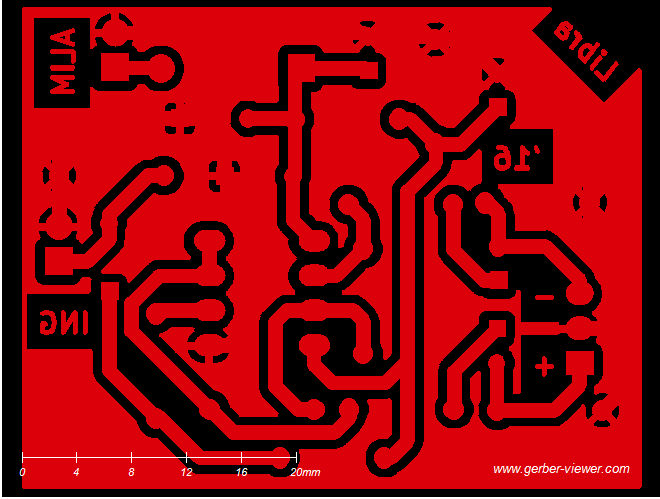
\includegraphics[scale=0.3]{img/real_world.png}
	\caption{The real world example used.}
\end{figure}

\subsection{Instance Generator}
\label{sec:instance:generator}
In order to provide some particular instances, I wrote a program that can be found in the folder
\verb|InstanceGenerator|. The usage is straightforward: you have to provide N, the number of points and
one letter out of \verb|r,c,q| which stands respectively for random, circle, square\footnote{If no option is provided the random option will be considered.}. The board is square-shaped with a fixed size of $10*N$.
\begin{itemize}
	\item If the option random is provided, it creates randomly $N$ points.
	\item if the option circle is provided, it creates 4 circles of $\lfloor{N/4}\rfloor$ points in the top-left, top-right, bottom-left, bottom-right corner
	of the drill board. If $N\ \text{mod} \ 4 = a$ with $a \neq 0$ then the circles $0..a$ will have $\lfloor{N/4}\rfloor + 1$ points.
	\item if the option square is provided, it creates 4 square of $\lfloor{N/4}\rfloor$ points in the top-left, top-right, bottom-left,
	bottom-right corner of the drill board. If $N$ is not a multiple of $4$, it tries to put the extra points somewhere inside the square.
\end{itemize}
In order to visualize the generated instances the files
\verb!/tmp/tsp_instance_<N>.gbr! and \verb!/tmp/tsp_instance_<N>.pbm!\footnote{This file format is a good choice because it is easy to encode 1 bit corresponds to 1 pixel, with 0 = white and 1 = black and is portable} are generated.
The latter file can be opened by each image viewer.
The instance generator program computes also a \verb|.dat| file containing the costs from drill point $i$ to drill point $j$.

The square and circle instances are very similar because they create instances in which the points are clustered on the corners.
But the circle instances are more flexible because they work well even with N that are not multiple of 4. Therefore they are used in the benchmark.
The advantage of the circle instances with respect to random generation is that the are reproducible the second not.